% Copyright (C) 2005-2015 Airbus - EDF - IMACS - Phimeca
% Permission is granted to copy, distribute and/or modify this document
% under the terms of the GNU Free Documentation License, Version 1.2
% or any later version published by the Free Software Foundation;
% with no Invariant Sections, no Front-Cover Texts, and no Back-Cover
% Texts.  A copy of the license is included in the section entitled "GNU
% Free Documentation License".
\renewcommand{\etapemethodo}{B}
\renewcommand{\nomfichier}{docref_B231_Pearson}
\renewcommand{\titrefiche}{Pearson Correlation Coefficient}

\Header


\MathematicalDescription{
  \underline{\textbf{Goal}} \vspace{2mm}

  This method deals with the parametric modelling of a probability distribution for a random vector $\vect{X} = \left( X^1,\ldots,X^{n_X} \right)$. It aims to measure a type of dependence (here a linear correlation) which may exist between two components $X^i$ and $X^j$.
  \vspace{2mm}

  \underline{\textbf{Principle}} \vspace{2mm}

  The Pearson's correlation coefficient $\rho_{U,V}$  aims to measure the strength of a linear relationship between two random variables $U$ and $V$. It is defined as follows:
  \begin{align*}
    \rho_{U,V} = \frac{\displaystyle \Cov{U,V}}{\sigma_U \sigma_V}
  \end{align*}
  where $\Cov{U,V} = \Expect{ \left( U - m_U \right) \left( V - m_V \right) }$, $m_U= \Expect{U}$, $m_V= \Expect{V}$, $\sigma_U= \sqrt{\Var{U}}$  and  $\sigma_V= \sqrt{\Var{V}}$. If we have a sample made up of a set of $N$ pairs $\left\{ (u_1,v_1),(u_2,v_2),\ldots,(u_N,v_N) \right\}$, Pearson's correlation coefficient can be estimated using  the formula:
  \begin{align*}
    \widehat{\rho}_{U,V} = \frac{ \displaystyle \sum_{i=1}^N \left( u_i - \overline{u} \right) \left( v_i - \overline{v} \right) }{ \sqrt{\displaystyle \sum_{i=1}^N \left( u_i - \overline{u} \right)^2 \left( v_i - \overline{v} \right)^2} }
  \end{align*}
  where $\overline{u}$  and  $\overline{v}$ represent the empirical means of the samples $(u_1,\ldots,u_N)$ and $(v_1,\ldots,v_N)$.

  Pearson's correlation coefficient takes values between -1 and 1. The closer its absolute value is to 1, the stronger the indication is that a linear relationship exists between variables $U$ and $V$.
  The sign of Pearson's coefficient indicates if the two variables increase or decrease in the same direction (positive coefficient) or in opposite directions (negative coefficient). We note that a correlation coefficient equal to 0 does not necessarily imply the independence of variables $U$ and $V$: this property is in fact theoretically guaranteed only if $U$ and $V$ both follow a Normal distribution. In all other cases, there are two possible situations in the event of a zero Pearson's correlation coefficient:
  \begin{itemize}
  \item the variables $U$ and $V$ are in fact independent,
  \item or a non-linear relationship exists between $U$ and $V$.
  \end{itemize}

  \begin{center}
    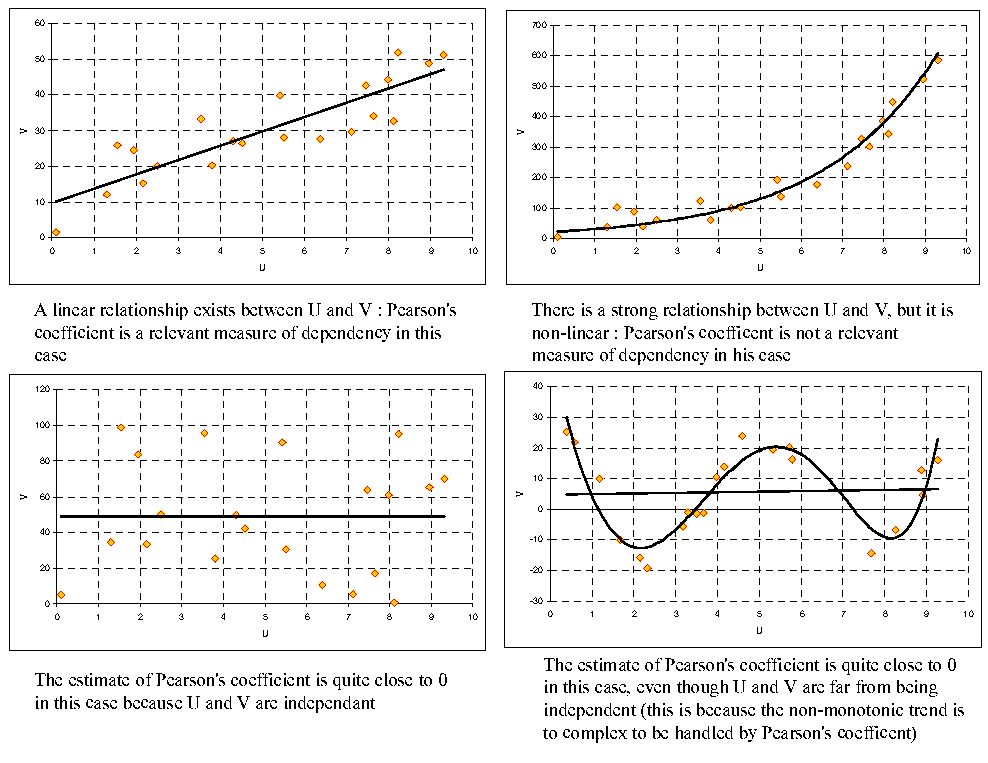
\includegraphics[width=0.5\textwidth]{Figures/pearson.pdf}
  \end{center}
}
{
  The estimate $\widehat{\rho}$ of Pearson's correlation coefficient is sometimes denoted by $r$.
}


\Methodology{
  Pearson's correlation coefficient can be used in step B "Quantifying Sources of Uncertainty". Having defined the vector $\underline{X}$ of input variables in step A "Specifying Criteria and the Case Study", \otref{docref_B231_TestPearson}{Pearson's Independence Test} shows how to test for the existence of a linear type of dependency between two components $X^i$ and $X^j$.
  Such a relationship should in fact be taken in to account so as not to falsify the results of step C "Propagation of Uncertainty".


  Pearson's correlation coefficient is also used in step C' "Sensitivity Analysis and Ranking of Sources of Uncertainty". If a propagation of uncertainty with Monte-Carlo simulation (step C, \otref{docref_C221_MonteCarloStd}{Mean and Variance Estimation using Standard Monte Carlo}) has been carried out, \otref{docref_Cprime212_Pearson}{Pearson's Ranking} shows the user how to class the components of the input vector $\underline{X}$ according to their impact on the uncertainty of a final variable / output variable defined in step A.

}
{
  Regardless of the method used in step B or step C', we recall that the Pearson's coefficient is only useful in measuring a linear relationship between two variables. Readers are referred to the following references:
  \begin{itemize}
  \item Saporta, G. (1990). "Probabilités, Analyse de données et Statistique", Technip
  \item Dixon, W.J. \& Massey, F.J. (1983) "Introduction to statistical analysis (4th ed.)", McGraw-Hill
    % \item NIST/SEMATECH e-Handbook of Statistical Methods, http://www.itl.nist.gov/div898/handbook/
    % \item D'Agostino, R.B. and Stephens, M.A. (1986). "Goodness-of-Fit Techniques", Marcel Dekker, Inc., New York.
  \item Bhattacharyya, G.K., and R.A. Johnson, (1997). "Statistical Concepts and Methods", John Wiley and Sons, New York.
    % \item Sprent, P., and Smeeton, N.C. (2001). "Applied Nonparametric Statistical Methods -- Third edition", Chapman \& Hall
    % \item Burnham, K.P., and Anderson, D.R (2002). "Model Selection and Multimodel Inference: A Practical Information Theoretic Approach", Springer
  \end{itemize}
}
